\subsection{FAtiMA}
\label{sec:fatima}
\ac{FAtiMA}\footnote{The toolkit is available at https://github.com/GAIPS-INESC-ID/FAtiMA-Toolkit.} is an agent architecture with planning capabilities designed to use emotions and personality to influence the agent's behaviour \cite{dias:fatima-modular}.
It has been used in different scenarios (\cite{paiva:learning-by-feeling},\cite{rodrigues:i-can-feel-to}, \cite{aylett:intercultural-empathy}, and \cite{correia:sueca}) and it is based on appraisal theory \footnote{The theory that emotions are elicited by evaluations (appraisals) of events and situations \cite{roseman:appraisal}.}.

\ac{FAtiMA} has a modular architecture where functionalities and processes are divided into modular independent components.
This enables users to use a lighter and simpler version of \ac{FAtiMA} by adding the required components to the \ac{FAtiMA} Core.

However, \ac{FAtiMA} Core does not commit itself with the particular methods used.
In fact a FAtiMA agent that only has a Core will not do anything.
Behaviour is added by adding components that implement the mentioned functionality.

Currently, \ac{FAtiMA} counts several already defined modules which the user can use out of the box (e.g. Cultural Behaviour \cite{mascarenhas:cultural-behaviour} and Drives \cite{lim:affective-npcs}, among others) but it can also write new modules to add different functionality to the model.
The architecture of \ac{FAtiMA} Core can be seen in Fig. \ref{fig:fatima-core}

\begin{figure}
  \centering
    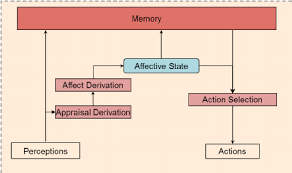
\includegraphics[width=.8\textwidth]{fatima-core}
  \caption{\ac{FAtiMA} Core's architecture.}
  \label{fig:fatima-core}
\end{figure}

An agent is able to receive perceptions from the environment (events) which are used to update the agent's memory (or internal state) and to trigger the appraisal process.
The result of the appraisal process is stored in the affective state, and later used to influence the action selection processes which will make the agent act upon the environment.
Appraisal Derivation is responsible for evaluating the relevance of the event to the agent and determines a set of appraisal variables and affect derivation takes these variables as input to generate the resulting affective states (emotions or mood).

As I said before, an agent using the \ac{FAtiMA} Core on its own will do nothing.
Agency is achieved by adding several components (or modules) to the Core.
In the scenario described in \cite{mascarenhas:cultural-behaviour}, the author used the following components:

\begin{itemize}
\item \textbf{Reactive Component}: uses a set of emotional reaction rules to determine values of some appraisal variables.
\item \textbf{Deliberative Component}: handles goal-based behaviour and adds planning capabilities to the agent. It also uses the state of plans in memory to generate appraisal variables.
\item \textbf{OCCAffectDerivation Component}: generates emotions from the appraisal variables according to the OCC Theory of Emotions \cite{ortony:occ}.
\item \textbf{Motivational Component}: models needs and goals for the agent that will influence the utility of a given goal.
\item \textbf{Theory of Mind Component}: creates a model of the internal states of other agents.
\item \textbf{Cultural Component}: implements cultural-dependent behaviour of agents through the use of rituals, symbols, and cultural dimensions, and determine the impact actions have on the motivational states of the agents.
\end{itemize}

\ac{FAtiMA} by itself is not a determined model for agency.
It is rather a framework that allows users to use whatever they need to achieve their goals.
In the given example, the result is a planning agent with cultural knowledge that uses emotions and personality to influence the planning of actions.

However the agent may not be social.
It has a mind reading capability, a required component for social ability (as seen in \ref{sec:social-agents}) but, empowering an agent with an emotional models does not make it social.
As previously described, actions must be themselves social in order for the agent to be social. 
Nonetheless, with its modular structure, \ac{FAtiMA} may be extended to encompass such social abilities.